\begin{tikzpicture}[x=1cm,y=1cm]
  \fill[infPaper] (-0.30,-17.05) rectangle (25.45,0.20);

  % COL 1: BRECHA Y HACER ESCUELA
  \draw[fill=white,draw=infNavy,line width=1.1pt,rounded corners=7pt] (0.0,-15.72) rectangle (8.15,0.0);
  \fill[infNavy,rounded corners=6pt] (0.0,-2.48) rectangle (8.15,0.0);
  \fill[infNavy] (0.0,-2.48) rectangle (8.15,-2.00);
  \node[anchor=north west,text width=5.45cm,align=left,inner sep=0pt] at (0.28,-0.22) {%
    {\color{white}\fontsize{11.5}{13.5}\selectfont\bfseries Philippe Meirieu (I)\par}\vspace{2pt}%
    {\color{white!90}\fontsize{7.3}{8.6}\selectfont\bfseries Crisis educativa, brecha y\\sentido de «hacer escuela»\par}\vspace{3pt}%
    {\colorbox{infBlueAccent}{\color{white}\fontsize{6.3}{7.3}\selectfont\bfseries\ Eje 1 · Institución y Bien Común \ }}%
  };
  \node[inner sep=0pt] at (6.92,-1.24) {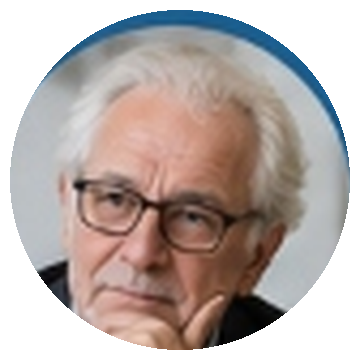
\includegraphics[width=2.06cm]{img_infografia/meirieu_photo.png}};

  \fill[infBlueLight] (0.12,-3.04) rectangle (8.03,-2.56);
  \node[font=\fontsize{6.9}{8.0}\selectfont\bfseries\color{infNavy}] at (4.075,-2.80) {«La escuela después»... ¿con la pedagogía de antes? (2020)};

  \InfSectionBar{0.20}{-3.16}{infNavy}{infBlueLight}{target}{Idea central del eje}
  \node[anchor=north west,text width=7.65cm,align=left,font=\fontsize{6.6}{8.0}\selectfont\color{infInk},inner sep=0pt] at (0.25,-3.74) {%
    Declarar «un antes y un después» es vano si el miedo y la inercia producen un «regreso a lo anormal». La escuela es institución pública donde se articula lo común y lo singular.%
  };

  \InfSectionBar{0.20}{-4.86}{infNavy}{infBlueLight}{key}{Conceptos clave}
  \InfConceptCard{0.20}{-5.44}{infNavy}{infBlueCard}{alerta}{\textbf{Brecha discurso}\\Coherencia real de prácticas.}
  \InfConceptCard{2.17}{-5.44}{infNavy}{infBlueCard}{escuela}{\textbf{Hacer el aula}\\Espacio-tiempo ritual común.}
  \InfConceptCard{4.14}{-5.44}{infNavy}{infBlueCard}{personas}{\textbf{«Yo» + «Nosotros»}\\Vínculo singular y colectivo.}
  \InfConceptCard{6.11}{-5.44}{infNavy}{infBlueCard}{libro}{\textbf{Saber compartible}\\Bienes sin agotamiento (Fichte).}

  \InfSectionBar{0.20}{-7.78}{infNavy}{infBlueLight}{bulb}{Tesis principales}
  \InfBullet{0.22}{-8.38}{infNavy}{Pregunta subversiva: \textit{«¿Por qué no hacemos lo que decimos que haremos?»} frente a rutinas excluyentes.}
  \InfBullet{0.22}{-9.04}{infNavy}{«Enseñar la clase» no es yuxtaponer apoyos individuales, sino sostener exigencia y bien común.}
  \InfBullet{0.22}{-9.70}{infNavy}{La escuela emancipa de determinismos familiares al abrir la alteridad y la palabra argumentada.}
  \InfBullet{0.22}{-10.36}{infNavy}{Los saberes matemáticos pertenecen a todos y se multiplican al compartirse sin perder valor.}

  \InfSectionBar{0.20}{-11.12}{infNavy}{infBlueLight}{gear}{Implicaciones en Matemáticas}
  \InfCheck{0.22}{-11.72}{infNavy}{Cuidar precisión verbal, unidades y verificación colectiva.}
  \InfCheck{0.22}{-12.26}{infNavy}{Construir normas de escucha donde ninguna pregunta sea burlada.}
  \InfCheck{0.22}{-12.80}{infNavy}{Evitar el aislamiento silencioso de series repetitivas mecánicas.}
  \InfCheck{0.22}{-13.34}{infNavy}{Asumir la clase técnica como comunidad de saber riguroso.}

  \fill[infBlueLight,rounded corners=5pt] (0.20,-15.52) rectangle (7.95,-14.05);
  \node[text width=7.35cm,align=center,font=\fontsize{6.6}{8.1}\selectfont\color{infNavy}] at (4.075,-14.78) {%
    \textbf{\textit{«El reto es evitar que el regreso a la normalidad sea un regreso a lo anormal competitivo.»}}\\
    {\scriptsize — Eje institucional · Meirieu (2020)}%
  };

  % COL 2: CRITICA TECNOCRATICA Y PEDAGOGIAS COOPERATIVAS
  \draw[fill=white,draw=infGreen,line width=1.1pt,rounded corners=7pt] (8.50,-15.72) rectangle (16.65,0.0);
  \fill[infGreen,rounded corners=6pt] (8.50,-2.48) rectangle (16.65,0.0);
  \fill[infGreen] (8.50,-2.48) rectangle (16.65,-2.00);
  \node[anchor=north west,text width=5.45cm,align=left,inner sep=0pt] at (8.78,-0.22) {%
    {\color{white}\fontsize{11.5}{13.5}\selectfont\bfseries Philippe Meirieu (II)\par}\vspace{2pt}%
    {\color{white!90}\fontsize{7.3}{8.6}\selectfont\bfseries Crítica tecnocrática y\\pedagogías cooperativas\par}\vspace{3pt}%
    {\colorbox{infGreenAccent}{\color{white}\fontsize{6.3}{7.3}\selectfont\bfseries\ Eje 2 · Tecnología y Cooperación \ }}%
  };
  \node[inner sep=0pt] at (15.42,-1.24) {
\includegraphics[width=2.06cm]{img_infografia/meirieu_illus.png}};

  \fill[infGreenLight] (8.62,-3.04) rectangle (16.53,-2.56);
  \node[font=\fontsize{6.9}{8.0}\selectfont\bfseries\color{infGreen}] at (12.575,-2.80) {Lo digital al servicio del vínculo humano, no del aislamiento};

  \InfSectionBar{8.70}{-3.16}{infGreen}{infGreenLight}{target}{Idea central del eje}
  \node[anchor=north west,text width=7.65cm,align=left,font=\fontsize{6.6}{8.0}\selectfont\color{infInk},inner sep=0pt] at (8.75,-3.74) {%
    Digitalizar una pedagogía transmisiva o conductista no innova: aisla al alumno frente a una pantalla. Las pedagogías cooperativas garantizan que nadie acapare ni sea excluido.%
  };

  \InfSectionBar{8.70}{-4.86}{infGreen}{infGreenLight}{key}{Conceptos clave}
  \InfConceptCard{8.70}{-5.44}{infGreen}{infGreenCard}{alerta}{\textbf{Conductismo digital}\\Software individual sin diálogo.}
  \InfConceptCard{10.67}{-5.44}{infGreen}{infGreenCard}{dialogo}{\textbf{Ayuda mutua}\\Cooperación frente a rivalidad.}
  \InfConceptCard{12.64}{-5.44}{infGreen}{infGreenCard}{autonomia}{\textbf{Ocupar su lugar}\\Participación equitativa de todos.}
  \InfConceptCard{14.61}{-5.44}{infGreen}{infGreenCard}{construccion}{\textbf{Mediación presencial}\\El encuentro cara a cara guía.}

  \InfSectionBar{8.70}{-7.78}{infGreen}{infGreenLight}{bulb}{Tesis principales}
  \InfBullet{8.72}{-8.38}{infGreen}{Alerta contra lógicas comerciales que reducen el aprendizaje a consumo privado de ejercicios.}
  \InfBullet{8.72}{-9.04}{infGreen}{La «cultura de resultados» concibe al maestro como simple aplicador o estorbo; urge defensa profesional.}
  \InfBullet{8.72}{-9.70}{infGreen}{Las pedagogías institucionales y cooperativas organizan roles rotativos donde cada voz cuenta.}
  \InfBullet{8.72}{-10.36}{infGreen}{La herramienta tecnológica solo vale si habilita indagación común, contraste gráfico y debate.}

  \InfSectionBar{8.70}{-11.12}{infGreen}{infGreenLight}{gear}{Implicaciones en Matemáticas}
  \InfCheck{8.72}{-11.72}{infGreen}{Contrastar salidas digitales en GeoGebra con análisis manual.}
  \InfCheck{8.72}{-12.26}{infGreen}{Alternar vocerías de equipo en sustentación de modelos.}
  \InfCheck{8.72}{-12.80}{infGreen}{Evaluar tanto el razonamiento propio como el aporte al grupo.}
  \InfCheck{8.72}{-13.34}{infGreen}{Priorizar comprensión física antes que velocidad de cálculo.}

  \fill[infGreenLight,rounded corners=5pt] (8.70,-15.52) rectangle (16.45,-14.05);
  \node[text width=7.35cm,align=center,font=\fontsize{6.6}{8.1}\selectfont\color{infGreen}] at (12.575,-14.78) {%
    \textbf{\textit{«Cuestionemos siempre qué relación con el saber y con los otros organiza cada herramienta digital.»}}\\
    {\scriptsize — Eje cooperativo · Meirieu (2020)}%
  };

  % COL 3: DERECHO EFECTIVO Y MUNDO DE TESOROS
  \draw[fill=white,draw=infOrange,line width=1.1pt,rounded corners=7pt] (17.00,-15.72) rectangle (25.15,0.0);
  \fill[infOrange,rounded corners=6pt] (17.00,-2.48) rectangle (25.15,0.0);
  \fill[infOrange] (17.00,-2.48) rectangle (25.15,-2.00);
  \node[anchor=north west,text width=5.45cm,align=left,inner sep=0pt] at (17.28,-0.22) {%
    {\color{white}\fontsize{11.5}{13.5}\selectfont\bfseries Philippe Meirieu (III)\par}\vspace{2pt}%
    {\color{white!90}\fontsize{7.3}{8.6}\selectfont\bfseries Derecho efectivo a aprender\\y «mundo de tesoros»\par}\vspace{3pt}%
    {\colorbox{infOrangeAccent}{\color{white}\fontsize{6.3}{7.3}\selectfont\bfseries\ Eje 3 · Equidad y Rodeo \ }}%
  };
  \node[inner sep=0pt] at (23.92,-1.24) {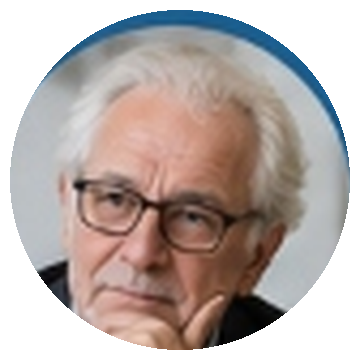
\includegraphics[width=2.06cm]{img_infografia/meirieu_photo.png}};

  \fill[infOrangeLight] (17.12,-3.04) rectangle (25.03,-2.56);
  \node[font=\fontsize{6.9}{8.0}\selectfont\bfseries\color{infOrange}] at (21.075,-2.80) {De la selección por prerrequisitos a «dar mejor»};

  \InfSectionBar{17.20}{-3.16}{infOrange}{infOrangeLight}{target}{Idea central del eje}
  \node[anchor=north west,text width=7.65cm,align=left,font=\fontsize{6.6}{8.0}\selectfont\color{infInk},inner sep=0pt] at (17.25,-3.74) {%
    Dejemos de convertir objetivos educativos en filtros de entrada. Ante la dificultad, la escuela justa ofrece «algo más» —rodeo didáctico— y abre un «mundo de tesoros» colaborativo.%
  };

  \InfSectionBar{17.20}{-4.86}{infOrange}{infOrangeLight}{key}{Conceptos clave}
  \InfConceptCard{17.20}{-5.44}{infOrange}{infOrangeCard}{balanza}{\textbf{Derecho vs. ocasión}\\Igualdad real de aprendizaje.}
  \InfConceptCard{19.17}{-5.44}{infOrange}{infOrangeCard}{target}{\textbf{Metas, no filtros}\\Entrenar antes de evaluar.}
  \InfConceptCard{21.14}{-5.44}{infOrange}{infOrangeCard}{andamio}{\textbf{«Algo más»}\\Rodeo frente a «más igual».}
  \InfConceptCard{23.11}{-5.44}{infOrange}{infOrangeCard}{lupa}{\textbf{Mundo de tesoros}\\Curiosidad frente a consumo.}

  \InfSectionBar{17.20}{-7.78}{infOrange}{infOrangeLight}{bulb}{Tesis principales}
  \InfBullet{17.22}{-8.38}{infOrange}{Rechazar el «síndrome del hospital» de la Carta a una profesora (Barbiana, 1967): no descartar a quien más apoyo requiere.}
  \InfBullet{17.22}{-9.04}{infOrange}{Aumentar dosis de idénticos ejercicios («más de lo mismo») profundiza el bloqueo; urge diagnóstico presencial.}
  \InfBullet{17.22}{-9.70}{infOrange}{Superar el taylorismo escolar y construir ecología sustantiva, no proyectos «suplemento de alma».}
  \InfBullet{17.22}{-10.36}{infOrange}{Sustituir un «mundo de tiendas» competitivo por un «mundo de tesoros» donde \textit{«nada se juega definitivamente»}.}

  \InfSectionBar{17.20}{-11.12}{infOrange}{infOrangeLight}{gear}{Implicaciones en Matemáticas}
  \InfCheck{17.22}{-11.72}{infOrange}{Cambiar representación verbal o gráfica cuando el despeje falla.}
  \InfCheck{17.22}{-12.26}{infOrange}{Valorar preguntas de diagnóstico sobre «matemáticas ingenuas».}
  \InfCheck{17.22}{-12.80}{infOrange}{Ofrecer segundas versiones tras retroalimentación formativa.}
  \InfCheck{17.22}{-13.34}{infOrange}{Conectar CONALEP, CECyTE e ingeniería con justicia educativa.}

  \fill[infOrangeLight,rounded corners=5pt] (17.20,-15.52) rectangle (24.95,-14.05);
  \node[text width=7.35cm,align=center,font=\fontsize{6.6}{8.1}\selectfont\color{infOrange}] at (21.075,-14.78) {%
    \textbf{\textit{«Porque nada, nunca, se juega definitivamente: todo estudiante tiene derecho a comprender.»}}\\
    {\scriptsize — Eje ético · Meirieu (2020)}%
  };

  % PIE DE FUENTE Y CREDITOS
  \draw[fill=infNavy,draw=infNavy,rounded corners=6pt] (0.0,-16.92) rectangle (25.15,-15.88);
  \node[inner sep=0pt] at (0.72,-16.40) {\InfIconOutline[0.36]{libro}{white}};
  \node[anchor=west,text width=16.8cm,align=left,font=\fontsize{6.6}{8.0}\selectfont\color{white}] at (1.30,-16.40) {%
    \textbf{FUENTE BASE (APA 7):} Meirieu, P. (2020, 18 de abril). \textit{«La escuela después»... ¿con la pedagogía de antes?} Movimiento Cooperativo de Escuela Popular (MCEP de Madrid; trad. de \textit{Café pédagogique}). \url{https://www.mcep.es/la-escuela-despues-con-la-pedagogia-de-antes-philippe-meirieu/}%
  };
  \node[anchor=east,text width=6.4cm,align=right,font=\fontsize{6.1}{7.4}\selectfont\color{white!90}] at (24.90,-16.40) {%
    \textbf{Mtro. Martín Jonathan de la Cruz Muñoz (Matrícula 00874)}\\
    IIIEPE · MAEM · Cohorte SD26 · Actividad 3 (Módulo 51440)%
  };
\end{tikzpicture}